%% ****** Start of file apstemplate.tex ****** %
%%
%%
%%   This file is part of the APS files in the REVTeX 4 distribution.
%%   Version 4.1r of REVTeX, August 2010
%%
%%
%%   Copyright (c) 2001, 2009, 2010 The American Physical Society.
%%
%%   See the REVTeX 4 README file for restrictions and more information.
%%
%
% This is a template for producing manuscripts for use with REVTEX 4.0
% Copy this file to another name and then work on that file.
% That way, you always have this original template file to use.
%
% Group addresses by affiliation; use superscriptaddress for long
% author lists, or if there are many overlapping affiliations.
% For Phys. Rev. appearance, change preprint to twocolumn.
% Choose pra, prb, prc, prd, pre, prl, prstab, prstper, or rmp for journal
%  Add 'draft' option to mark overfull boxes with black boxes
%  Add 'showpacs' option to make PACS codes appear
%  Add 'showkeys' option to make keywords appear
%\documentclass[aps,prl,preprint,groupedaddress]{revtex4-1}
\documentclass[aps,prl,preprint,superscriptaddress]{revtex4}
%\documentclass[aps,prl,reprint,groupedaddress]{revtex4-1}

% You should use BibTeX and apsrev.bst for references
% Choosing a journal automatically selects the correct APS
% BibTeX style file (bst file), so only uncomment the line
% below if necessary.
%\bibliographystyle{apsrev4-1}
\usepackage{graphicx}
\usepackage{float}
\usepackage{subfig}
\usepackage{textcomp}
\usepackage[none]{hyphenat}
\setcounter{secnumdepth}{3}


\begin{document}

% Use the \preprint command to place your local institutional report
% number in the upper righthand corner of the title page in preprint mode.
% Multiple \preprint commands are allowed.
% Use the 'preprintnumbers' class option to override journal defaults
% to display numbers if necessary
%\preprint{}

%Title of paper
\title{The determination of Stokes constants for Schr\"{o}dinger equation with non-analytic potential}

% repeat the \author .. \affiliation  etc. as needed
% \email, \thanks, \homepage, \altaffiliation all apply to the current
% author. Explanatory text should go in the []'s, actual e-mail
% address or url should go in the {}'s for \email and \homepage.
% Please use the appropriate macro foreach each type of information

% \affiliation command applies to all authors since the last
% \affiliation command. The \affiliation command should follow the
% other information
% \affiliation can be followed by \email, \homepage, \thanks as well.
\author{Anton Kutlin}
%\email[]{Your e-mail address}
%\homepage[]{Your web page}
%\thanks{}
%\altaffiliation{}
\affiliation{Institute of Applied Physics of Russian Academy of Sciences, 46 Ulyanov str., 603950 Nizhny Novgorod, Russia}

%Collaboration name if desired (requires use of superscriptaddress
%option in \documentclass). \noaffiliation is required (may also be
%used with the \author command).
%\collaboration can be followed by \email, \homepage, \thanks as well.
%\collaboration{}
%\noaffiliation

\date{\today}

\begin{abstract}
In many cases of practical interest it is not necessary to know a solution of a differential equation precisely and enough to determine only some characteristics of the solution such as the absorption coefficient or energy eigenvalues. For this purpose in case of a differential equation of the Schr\"{o}dinger type the method of Phase Integrals is commonly used. A cornerstone of the method is the Stokes constants. There are a very few cases in which it is possible to determine the constants precisely, so approximate methods must be used. If the solution does not have any branch points it is possible to write equations for the constants using analytical continuation around the origin and requiring the solution to be single valued. This can be done in case of a single algebraic branch point with minor variations, but it is still difficult to do this when the solution has an infinite number of sheets or several branch points. The present work is devoted to demonstrate some ideas regarding this problem.
\end{abstract}

% insert suggested PACS numbers in braces on next line
\pacs{}
% insert suggested keywords - APS authors don't need to do this
\keywords{Method of Phase Integrals, WKB, WKBJ, Stokes phenomenon, Stokes constants, the Budden problem, symmetry relations, Frobenius series, branching structure}

%\maketitle must follow title, authors, abstract, \pacs, and \keywords
\maketitle

\section{introduction \label{intro}}
Every linear second-order ordinary differential equation can be put in the Schr\"odinger form:
\begin{eqnarray}
\frac{d^2y}{dz^2} + Q(z,\lambda)y = 0,   \label{wkbeqn}
\end{eqnarray}
where \mbox{$Q(z,\lambda)$} will be referred to as a potential. For example, in case of a simple quantum harmonic oscillator and an energy eigenvalue problem \mbox{$Q(z,E)=E-z^2$}. Briefly, the WKBJ (and often simply WKB) 
approximate solutions of Eq.\ref{wkbeqn}, so named after
Wentzel, Kramers, Brillouin, and Jeffreys\cite{wkbj}, take the form
\begin{eqnarray}
y_\pm = Q^{-1/4} e^{\pm i \int^z Q^{1/2} dz},   \label{wkbsol}
\end{eqnarray}
and provided that
$\left|\frac{dQ}{dz}Q^{-3/2}\right| \ll 1 $
a general solution of Eq.~\ref{wkbeqn} can be approximated by
\begin{eqnarray}
y = a_+y_+ + a_-y_-.    \label{gensol}
\end{eqnarray}
Clearly the inequality is not valid in a vicinity of poles and zeros of the potential. Such points will be referred to as singular points and the vicinity of a singularity will be referred to as the interaction area.

According to Stokes\cite{stokes}, coefficients $a_+$ and $a_-$ in Eq. (\ref{gensol}) differ from one domain of the complex plane to another. Such changes happen on so-called Stokes lines and have a form of a single-parameter linear transform\cite{heading}. The parameter associated with a particular Stokes line is called the Stokes constant. Knowing all Stokes constants associated with a particular potential gives an ability to obtain a globally defined approximate solution of Eq.~\ref{wkbeqn}\cite{heading,rwbook}.

For an isolated singular point with $Q$ analytic, the Stokes constant 
can be determined by a continuation around the complex plane, requiring the WKB approximation to be single valued.
This gives\cite[p.~83]{rwbook} for $Q = z^n$, the value $S = 2icos(\pi/(n+2))$.

For several singular points associated with an analytic potential it is still possible to require the function to be  single valued to obtain equations for Stokes constants. But in this case it can be impossible to determine all the constants or sometimes the information about their phase can be incorrect\cite[pp~243-245]{rwbook}.

Solutions of equation (\ref{wkbeqn}) with a non-analytic potential are not single valued and usually have both algebraic and logarithmic branch points, so there is no possibility of requiring the function to be single valued to write equations for the Stokes constants. The approximation of using Stokes constants  for isolated singularities can give an estimate, but the results are correct only in the limit of large separation of singularities. Inasmuch as the most interesting cases from the physical point of view often imply small separation, this problem needs further investigation.

The simplest example of an equation with a non-analytic potential is the Budden potential.
In section \ref{budden} the potential is studied using the approximation of isolated singularities and compared with an exact solution.  
In section \ref{frob} the possibility of using a local series expansion to achieve an equation for the Stokes constants is discussed. 
In section \ref{symmetries} symmetry relations are found which can relate different Stokes constants.
In section \ref{summury} transmission and absorption values for the Budden problem are given without obtaining the solution of the differential equation.
And, finally, in section \ref{con} are the conclusions. 

\section{The Budden Problem \label{budden}}

We consider the standard problem treating the penetration and resonant absorption of an electromagnetic wave, analyzed by Budden\cite{white-chen,budden}. The differential equation is
\begin{eqnarray}
\frac{d^2y}{dz^2} + (1+c/z)y = 0.  \label{budeq}
\end{eqnarray}
The Budden potential has a first order zero or cutoff  at \mbox{$z=-c$} and a resonance or first order pole at \mbox{$z=0$}. One can find that the pole should be rounded from below. This condition is equivalent to the Landau prescription for the pole to describe Landau
damping. Note that the singularity at \mbox{$z=-c$} is an artifact of the WKBJ
analysis. The differential equation has only a pole at \mbox{$z=0$}, and thus a
single cut of the solution extending upward from this point.

The Budden problem is a problem of determination of the absorption in the Budden potential. It can be solved exactly using an integral representation. A detailed  analysis of the problem can be found in \cite[pp~230-235]{rwbook}. Since the aim of this paper is to discuss asymptotic methods of solving such problems, a solution of the Budden problem using an approximation of isolated singularities is shown below.

Following \cite{heading}, define \mbox{$(a,z) = Q^{-1/4}e^{i\int_a^z Q^{1/2} dz}$} and \mbox{$[a,b] = e^{i\int_a^b Q^{1/2} dz}$}. Corresponding with (\ref{wkbsol}), the equation (\ref{budeq}) has \mbox{$y_+=e^{iz}$} and \mbox{$y_-=e^{-iz}$} as its WKBJ asymptotic.  Begin with a solution representing an outgoing wave at large positive $z$. According to \cite[p.~95]{rwbook}, using the approximation of isolated singularities one can obtain for \mbox{$Arg(z)=-\pi$} that
\begin{eqnarray}
y=i([0,-c]+[-c,0]/2)(z,-c) +([0,-c]-[-c,0]/2)(-c,z).
\end{eqnarray}
Since \mbox{$[0,-c]=e^{\frac{\pi c}{2}}$}, reflection and transmission coefficients are
\begin{eqnarray}
R=-i\frac{2e^{\frac{\pi c}{2}}-e^{-\frac{\pi c}{2}}}{2e^{\frac{\pi c}{2}}+e^{-\frac{\pi c}{2}}},\ 
T=-i\frac{2}{2e^{\frac{\pi c}{2}}+e^{-\frac{\pi c}{2}}},
\end{eqnarray}
and for absorption
\begin{eqnarray}
A=1-|R|^2-|T|^2=\frac{4 e^{\pi c}}{(1+2e^{\pi c})^2}.
\end{eqnarray}

\begin{figure}
\centering
\noindent
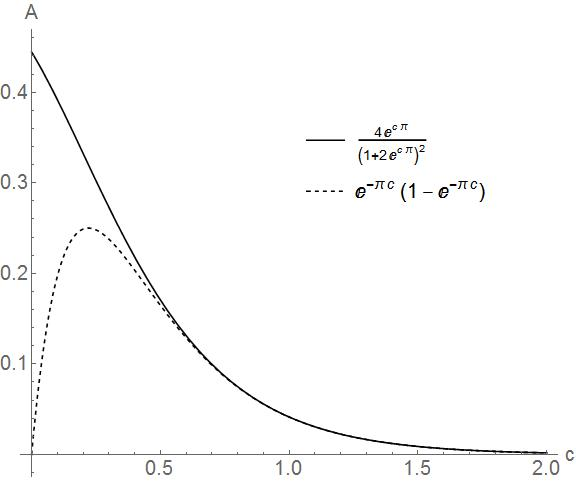
\includegraphics[scale=.5]{stuff/comparison.jpg}
\caption{Absorption in the Budden potential}
\label{cmprsn}
\end{figure} 

Comparing the expression with the one from an exact solution (see Fig.\ref{cmprsn}) it is easy to see that they behave similarly when \mbox{$c\geq1$}, but not when \mbox{$c\ll 1$}. The limit of \mbox{$c\rightarrow 0$} is clearly wrong; in this limit \mbox{$Q=1$}
and there should be no reflection or absorption. The error is due to using the Stokes constants which do not preserve the global structure of the solution with a branch point. In the next section we consider how to correct this. 

\section{Deriving an equation for the Stokes constants using a series representation \label{frob}}
The pole of the Budden potential is a regular singular point. It is a well known fact\cite[pp~68-76]{bender} that if \mbox{$z=0$} is a regular singular point of $Q(z)$ than the general solution of Eq.\ref{wkbeqn} can be written in the form
\begin{eqnarray}
y=A y_1+B y_2=
Az^{f_1}\sum_{n=0}^{\infty}{a_n z^n}+B(z^{f_2}\sum_{n=0}^{\infty}{b_n z^n}+Kln(z)z^{f_1}\sum_{n=0}^{\infty}{a_n z^n}),    \label{frobgensol}
\end{eqnarray}
where $A$ and $B$ are arbitrary constants and $K$ is to be determined. This is the Frobenius form, and solving differential equations this way called the Frobenius method. The constant $K$ and coefficients of the Taylor series can be determined by direct substitution of the solution into the differential equation. Since \mbox{$z=0$} is the only pole of the potential the Taylor series have infinite radii of convergence. Constants $f_1$ and $f_2$ are called Frobenius indexes and are determined by the characteristic equation
\begin{eqnarray}
f(f-1)+\lim_{z\rightarrow 0}(z^2Q(z))=0.   \label{chareq}
\end{eqnarray}
In case of the Budden potential, the general solution is
\begin{eqnarray}
y=A z \sigma_1(z)+B(\sigma_2(z) - c ln(z)z\sigma_1(z)),   \label{genfrobbud}
\end{eqnarray}
where $\sigma$ stands for a Taylor series. There is a single valued solution \mbox{$A z \sigma_1(z)$}. It does not matter how $A$ is connected with $a_+$ and $a_-$ from (\ref{gensol}), it is only important that there are such coefficients which represent a solution without a logarithmic branch point. This can be used to write an equation for the Stokes constants because continuing analytically around the origin from \mbox{$Arg(z)=0$} to \mbox{$Arg(z)=2\pi$} this solution is  multiplied by 1! In the general case the solution may not be single valued,and  a solution should be multiplied by $e^{2i\pi f_1}$ instead of $1$. In other words, a matrix representing complete rotation around the origin should have $e^{2i\pi f_1}$ as its eigenvalue. 

\begin{figure}
\centering
\noindent
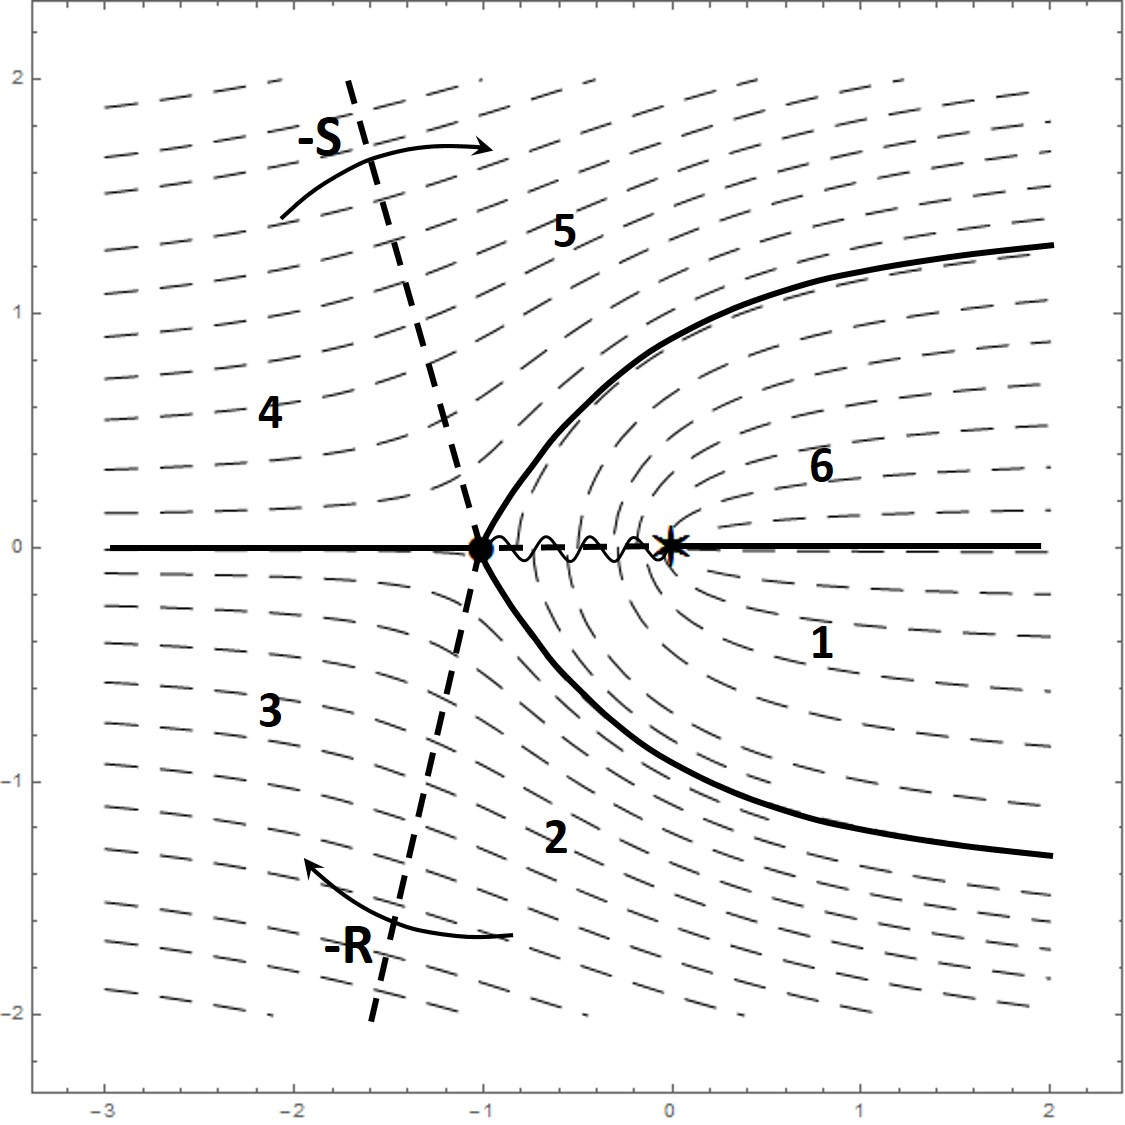
\includegraphics[scale=.5]{stuff/diagram.jpg}
\caption{Stokes diagram for the Budden problem; Stokes lines are bold and dashed}
\label{diagram}
\end{figure} 

Using the information from the Frobenius method it is now possible to write an equation for the Stokes constants for the Budden potential. To continue the general solution analytically around the origin let's place the cut between \mbox{$z=0$} and \mbox{$z=-c$} along the real axis as shown on Fig.\ref{diagram}. Starting with \mbox{$y=a_+e^{iz}+a_-e^{-iz}$} from large $|z|$ and \mbox{$Arg(z)=0$} and using the rules for continuation from \cite[pp 83-84]{rwbook}, one can obtain that the continuation is \\
$1.\ a_+(0,z)_d+a_-(z,0)_s=a_+[0,-c](-c,z)_s + a_-(z,-c)_d[-c,0]$\\
$2.\ a_+[0,-c](-c,z)_d + a_-[-c,0](z,-c)_s$\\
$3.\ a_+[0,-c](-c,z)_d + (a_-[-c,0] - R a_+[0,-c])(z,-c)_s$\\
$4.\ a_+[0,-c](-c,z)_s + (a_-[-c,0] - R a_+[0,-c])(z,-c)_d$\\
$5.\ (a_-[-c,0] - R a_+[0,-c])(z,-c)_d + (a_+[0,-c]-S(a_-[-c,0] - R a_+[0,-c]))(-c,z)_s$\\
$6.\ (a_-[-c,0] - R a_+[0,-c])(z,-c)_s + (a_+[0,-c]-S(a_-[-c,0] - R a_+[0,-c]))(-c,z)_d$.

All integrals here were evaluated below the cut and give $[0,-c]=e^{\frac{\pi c}{2}}$. The unknown Stokes constants $R$ and $S$ were taken with minus sign because the Stokes lines were crossed in a clockwise sense. As it could be seen from an expression for \mbox{$y(|z|e^{-i\pi})$}, $R$ is an exact reflection coefficient for a wave incident from the left and $T$ is equal to $e^{-\frac{\pi c}{2}}$.
Finally, reconnecting from $z=-c$ to $z=0$ above the cut and identifying incoming and outcoming waves the solution for \mbox{$Arg(z)=-2\pi$} can be written as
\begin{eqnarray}
y(|z|e^{-2\pi i})=(-Sa_- +e^{c \pi}(1+RS)a_+)e^{i|z|}+(e^{-c \pi} a_- - R a_+)e^{-i|z|}.   \label{m2pirot}
\end{eqnarray}
Requiring $y(|z|e^{-2\pi i})$ to be equal to $y(|z|)$ one can obtain a linear system for $a_+$ and $a_-$. The condition for a solution to exist is
\begin{eqnarray}
RS=-(1-e^{-\pi c})^2.   \label{frobresult}
\end{eqnarray}

The values of the Stokes constants for isolated singularities can approximately satisfy expression (\ref{frobresult}) only for large values of $c$. This explains why the approximation from the previous section could not give a correct result for \mbox{$c\ll 1$}. But this still does not determine  the absorption coefficient because of unknown relations between $R$ and $S$. In the next section we derive such relations.

\section{Symmetry relations for Stokes constants \label{symmetries}}
The Budden potential is real on the real axis. This property implies special symmetry relations between the Stokes constants  and thereby reduces the number of independent Stokes constants.

Assume a solution in some domain of the complex plane is of the form (\ref{gensol}). The coefficients before the WKBJ solutions could be written as a two-dimensional vector
\[
\psi=\left( \begin{array}{c} a_+ \\ a_- \end{array} \right).
\]
Following \cite[pp~21-33]{froman}, the F-matrix is defined as a translation matrix acting on the vector of asymptotic coefficients, so
\[
\psi(z_2)=F(z_2,z_1)\psi(z_1).
\]

Far away from the interaction area it is convenient to choose a polar coordinate system and write $z$ as $|z| e^{i \phi}$.
According to \cite{symm} if \mbox{$\sqrt{Q(|z|e^{i \phi})}=\sqrt{Q^*(|z|e^{-i \phi})}$} then
\begin{eqnarray}
F(-\phi,-\phi_0)=
\left( \begin{array}{cc} 0 & 1 \\ 1 & 0 \end{array} \right)
F(\phi,\phi_0)^*
\left( \begin{array}{cc} 0 & 1 \\ 1 & 0 \end{array} \right)
    \label{fmatrsym1}
\end{eqnarray}
and if \mbox{$\sqrt{Q(|z|e^{i \phi})}=-\sqrt{Q^*(|z|e^{-i \phi})}$} then 
\begin{eqnarray}
F(-\phi,-\phi_0)=F(\phi,\phi_0)^*.
    \label{fmatrsym2}
\end{eqnarray}

For the Budden potential, one can find a relation between $R$ and $S$ using (\ref{fmatrsym1}) and writing
\begin{eqnarray}
F(-3\pi/2+\varepsilon,-3\pi/2-\varepsilon)=\left( \begin{array}{cc} 1 & S \\ 0 & 1 \end{array} \right), 
F(-\pi/2-\varepsilon,-\pi/2+\varepsilon)=\left( \begin{array}{cc} 1 & 0 \\ -R & 1 \end{array} \right).
\end{eqnarray}
The required relation is
\begin{eqnarray}
R=-S^*.    \label{desiredrel}
\end{eqnarray}

\section{Summary \label{summury}}

In section \ref{frob} a series expansion was used to find a relation which provides the correct global branching structure of the general solution. The relation is
\begin{eqnarray}
RS=-(1-e^{-\pi c})^2.  
\end{eqnarray}
Also, the analytical continuation gave an expression for the transmission coefficient:
\begin{eqnarray}
T=e^{-\frac{\pi c}{2}}.
\end{eqnarray}

In section \ref{symmetries} symmetry of the potential was used to reduce a number of independent Stokes constants. It was found that
\begin{eqnarray}
R=-S^*. 
\end{eqnarray}

Now one can finally write an expression for the absorption coefficient:
\begin{eqnarray}
A=1-|R|^2-|T|^2=1-(1-e^{-\pi c})^2-e^{-\pi c}=e^{-\pi c}(1-e^{-\pi c}).    \label{absorp}
\end{eqnarray}
The expression (\ref{absorp}) agrees with the analytical result obtained in \cite[p 234]{rwbook}.

\section{A case of an equation without an exact solution \label{UHR}}
The example of the Budden problem is, certainly, a rare example of the problem which can be completely solved. In most cases we will not be able to solve an equation analogous to Eq.\ref{frobresult} exactly because of large amount of unknowns and lack of other equations. But since such an equation is highly non trivial, it can be used to elucidate unobvious features of a solution even in a such situations. To illustrate it, let`s study the following equation:
\begin{eqnarray}
\frac{d^2y}{dz^2} + \frac{Y^2-z^2}{z}y = 0.  \label{uhreq}
\end{eqnarray}
Such an equation describes an absorption of an extraordinary electromagnetic wave in the vicinity of an upper-hybrid resonance providing the wave propagates along the electron concentration gradient and an external magnetic field is weak $(Y \ll 1)$. Physics of the process is irrelevant for the purpose of this paper so we allow $Y$ to take any values.

An effective Stokes diagram for Eq.\ref{uhreq} is shown on Fig.\ref{uhr_sd}. To obtain a brunching structure preserving equation, let`s find Frobenius indexes for Eq.\ref{uhreq}. According to Eq.\ref{chareq}, $f_1=0$ and $f_2=1$, and the equation is
\begin{eqnarray}
Tr(CS[s_+]W[w]S[s_0]W[-w^*]S[s_-])=2,  
\end{eqnarray}
or, using an explicit form of the operators,
\begin{eqnarray}
s_0e^{2Re(w)} + s_+e^{2iIm(w)} + s_-e^{-2iIm(w)} +s_-s_0s_+e^{2Re(w)}=2i.   \label{uhr_frob}
\end{eqnarray}

To reduce the number of independent unknowns we use a conjugation symmetry of Eq.\ref{uhreq} exactly as we did in a case of the Budden problem. A result is analogous and typical for an equation with the real-valued potential: $s_0=-s_0^*$, $s_+=-s_-^*$. Taking into consideration that the reflection and absorption coefficients in this case have the same expressions in terms of the Stokes constants as in the previous example, let`s define three independent real unknowns $p, \rho$ and $\phi$ by $s_0=2ip$ and $s_-=-\rho e^{i\phi}$. In terms of the new variables Eq.\ref{uhr_frob} can be rewritten as
\begin{eqnarray}
p (1-\rho^2) e^{2Re(w)} - \rho sin(\phi-2Im(w)) - 1 = 0,   \label{realFrobEq}
\end{eqnarray}
where $\rho=|R|$ and $\phi=Arg(R)$. It is simpler than the initial one, but it is still the only one equation with three real unknowns and it cannot be solved exactly.

Let's try to solve it in case of almost full reflection, $1-\rho \ll 1$. In this case we can express the absorption coefficient $A=1-|R|^2=1-\rho^2$ right away:
\begin{eqnarray}
A=p^{-1}(1 + sin(\phi-2Im(w)))e^{-2Re(w)}. \label{allRefl}
\end{eqnarray}
An assumption $1-\rho \ll 1$ induce a relation $A \ll 1$, and according to Eq.\ref{allRefl} this is true if $Re(w) \gg 1$. But this last inequality allows us to use an approximation of isolated singularities - in a limit of large values of $w$ $p$ approaches 1/2 and $\phi$ approaches $-\pi/2$, and
\begin{eqnarray}
A=4sin^2(Im(w))e^{-2Re(w)}.   \label{ais}
\end{eqnarray}
The expression shows how the absorption coefficient behaves for large values of $Y$. The most important feature of this result is a footprint of an interference in the system - there are strict zeros of absorption for $Im(w)=\pi n$. This non trivial result could not be obtained in another way - an approximation of isolated singularities ignores the interference because it knows nothing about the actual structure of the potential. A comparison of Eq.\ref{ais} with the numerical result and a simple approximation of isolated singularities is shown on Fig.\ref{uhr_comp}.





\section{Conclusion \label{con}}
The example of the Budden potential shows that use of a series representation of a solution gives an additional equation for the Stokes constants. Since the equation reflects actual branching structure of a general solution it can correctly describe the behaviour of the Stokes constants even in the case of non-isolated singularities. Also, different symmetries of a potential can be used to reduce the number of independent Stokes constants.

Certainly this does not guarantee that the relations discussed above are enough to determine all of the Stokes constants. It is possible to combine the ideas outlined in this paper with other approximation such as the use of constants for isolated singularities or isolated pairs of singularities.

\textbf{Acknowledgement}
The work is supported by the Russian Science Foundation (project \textnumero 15-02-07600-a). The author would like to express his immense grateful to Dr.~R.B.White for the assistance in writing this article and for his fascinating book about asymptotic analysis. He also thanks Dr.~E.D.Gospodchikov for discussions which finally led the author to the idea of writing this paper. Last but not least, the author shows his gratitude to his close friend, Mikhail Mlodik, for his constant support and useful advices.

\begin{thebibliography}{10}
\bibitem{wkbj} G. Wentzel, Zeit. f. Phys. 38, 518 (1926), H. A. Kramers,
 Zeit. f. Phys. 39, 828 (1926), L. Brillion, C. R. Acad. Sci. Paris 183, 
24 (1926), H. Jeffries, Philos. Mag. [7] 33, 451 (1942)
\bibitem{stokes} Stokes, G. G., Trans. Camb. Phil. Soc. 10, 105 (1857).
\bibitem{heading} J. Heading. {\it An Introduction to Phase Integral Methods} 
Wiley, NY (1962)
\bibitem{rwbook} R. B. White,
 {\it Asymptotic Analysis of Differential Equations}, Imperial College Press, 2010.
\bibitem{budden} Budden, K. G., Phil. Trans. Royal Soc. London 290, 405 (1979).
\bibitem{white-chen} White, R. B. and Chen, F. F., Plasma Physcis 16, 565 (1974).
\bibitem{bender} C. M. Bender, S. A. Orszag,
 {\it Advanced Mathematical methods for Scientists and Engineers}, Springer, 1999.
\bibitem{froman} Fr\"oman, N., Fr\"oman, P. O.,
 {\it Asymptotic Analysis of Differential Equations}, Cambrige University Press, 2004. 
\bibitem{symm} Fr\"oman, N., Fr\"oman, P. O., and Lundborg, B., 1988b, Math Proc Camb Phil Soc 104, 181–191
\end{thebibliography}
\end{document}